\bbsection{Use Cases}{use-cases}

\bbsubsection{Use Case Diagram}{use-case-diagram}
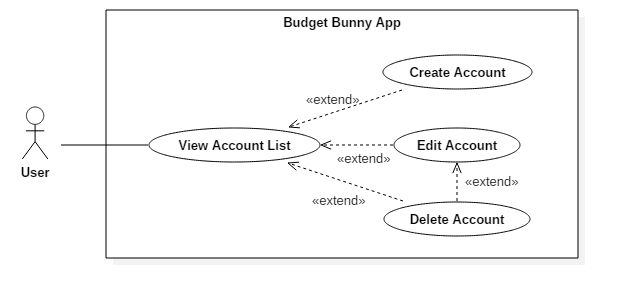
\includegraphics[scale=0.8]{use-case-diagram}

\bbsubsection{Use Case Description}{use-case-description}

Unless otherwise stated, the primary actor for all use cases is the user of the application, which shall simply be called, "User". Note: the Usage Frequency portion is inaccurate for now. Once the usage data has been gathered and collated, the Usage Frequencies of each use case will be updated.

\usecase{ACC-0001}
	{Create Account}
    {The user creates a new account, supplying its name, currency, and initial amount. All fields are required. The user may also set the newly created account as default.}
    {There are no pre-conditions.} %% There WILL be a precondition, once we add a check where we make sure that there is a maximum number of accounts.
    {The account is added into the core data.}
    {The user enters the name in alphanumeric characters, and the initial amount in numeric characters, both within the limits of the text field's length. The user then chooses the account's currency, and taps the Done button, saving the newly created account into the core data.}
    {
    ~ 
    \begin{itemize}
		\item All fields are required. When at least one field is not filled, an error alert will appear.
        \item Both the account name and the initial amount text fields have a limit in their length. When the user hits the limit and keys in a new character, the text field will not respond.
        \item On a related note, when the user pastes text into the text field with a length longer than the given limit, it will not respond as well.
        \item No two account names must be the same. An alert will be shown if the name already exists in the core data.
    \end{itemize}    
    }
    {N/A}
    
\usecase{ACC-0002}
	{View Account List}
    {The user views a list of all their accounts.}
    {There is at least one account in the core data available for viewing.}
    {The state and number of accounts before and after viewing stays the same.}
    {The user is able to view all their accounts.}
    {~
    \begin{itemize}
    	\item When the user swipes a non-default account cell to the left, two buttons appear, enabling the user to either mark the account as default, or delete the account.
        \item Default accounts cannot be deleted, nor can they be set as default again. When the user swipes a default account cell to the left, one button appears, enabling the user to edit the account. Ultimately, this means that there is always at least one account available for viewing.
        \item All table cells can be tapped. Once tapped, the user proceeds to the Edit Account Screen.
        \item If there are no accounts available for viewing, then the table will not be visible, containing a block of placeholder text in its place. This scenario is technically not possible, because upon installation of the app, placeholder accounts will be automatically created. 
    \end{itemize}
    }
    {N/A}
    
\usecase{ACC-0003-1}
	{Edit Account}
    {The user can edit the account's name, current amount, or the currency.}
    {There is at least one account in the core data available for editing.}
    {The user has updated the account that they wanted to edit.}
    {The user edits all the fields in the account --  the name, current amount, and the currency and taps save, updating the core data with the changes.}
    {~
    \begin{itemize}
    	\item If the account is not a default account, the user can set the account as default, or they can delete the account.
        \item All conditions in ACC-0001 apply here. Specifically, all fields are required, all fields have a character limit, and no two account names must be the same.
    \end{itemize}}
    {N/A}
    
\usecase{ACC-0003-2}
	{Delete Account}
    {The user will delete the account, removing it from the core data.}
    {There is at least one non-default account which is available for deletion.}
    {The non-default account is deleted, leaving one less account in the core data.}
    {The delete button can be located in either the Edit Account or the View Account List. Once tapped, an alert will be displayed, warning them that the action is destructive and cannot be undone. The user then taps the delete button, confirming the deletion.}
    {Once the confirmation alert is displayed, the user may tap the darkened area of the screen, or the cancel button to cancel the deletion.}
    {N/A}
